\section{System Design}
\label{sec:design}

\begin{figure*}[t]
  \centering
  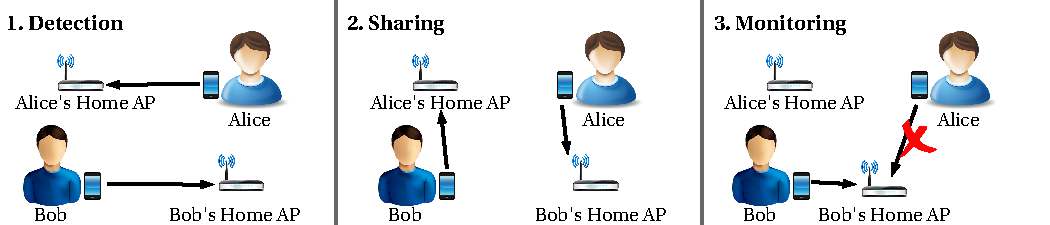
\includegraphics[width=\textwidth]{./figures/design.pdf}
  \caption{\textbf{\wisefi{} System Work Flow.} (1) Reciprocal sharing
    opportunities are detected by \wisefi{} smartphone apps; (2) \wifi{} sharing
    is enabled through coordination of \wisefi{} server; (3) \wifi{} usage and
    performance are monitored by \wisefi{} app to ensure the sharing remains
  reciprocal.}
  \label{fig:design}
\end{figure*}

Inspired by the results of the investigation in Section~\ref{sec:investigation},
we design a system called \wisefi{} to detect reciprocal sharing
opportunities (\S\ref{subsec:detection}), enable \wifi{} sharing
(\S\ref{subsec:sharing}) and monitor the \wifi{} performance to ensure the
sharing remains reciprocal (\S\ref{subsec:monitoring}). Figure~\ref{fig:design}
shows the overall work flow of the \wisefi{} system.

\subsection{Detection}
\label{subsec:detection}

To detect reciprocal sharing opportunities, two information are required: the
home AP of the device, and neighbor APs' signal strength during \wifi{} sessions
with the home AP. A smartphone application can be deployed through app market to
collect these information. In particular, the home AP information can be learned
over a period of time using the heuristics developed in
Section~\ref{subsec:homeap}, or be inputed directly by user. Once the home AP
information is identified, \wifi{} scan results during sessions with home APs
can then be logged to identify the neighbor APs that can potentially provide
better network performance. Finally, these information are uploaded and fused in
\wisefi{} server to identify reciprocal sharing opportunities using the methods
described in Section~\ref{subsec:reciprocal}.

\subsection{Sharing}
\label{subsec:sharing}

Once the reciprocal sharing opportunities are discovered, the \wisefi{} server
can distribute such information to the \wisefi{} application on smartphone,
which will prompt users to establish \wifi{} sharing. The sharing mechanism must
meet two goals: control and protection. First, the system should be able to
control the sharing, including granting the access of home AP to other \wisefi{}
users, and revoking the access when the reciprocal sharing opportunity no longer
exists.  Second, the system should protect the home network from other \wisefi{}
users by sharing access only to the Internet, and protecting private resources
such as home network printers or storage.

Some mid-to-high end wireless routers support the \textit{virtual network}
feature, where multiple virtual \wifi{} networks are emulated by a single router
hardware, and different network parameters, such as SSID, bandwidth cap, access
permission, can be enforced separately for each virtual network. This feature is
typically used to set up a guest \wifi{} network to provide network access to
temporal visitors yet isolate them from home clients. For home APs with such
feature, \wifi{} sharing can be achieved by only distributing the credential of
guest network to other \wisefi{} users. Access and bandwidth policies can then
be enforced on the guest network to achieve control and protection.
Additionally, such isolation and enforcements are mostly likely already enabled
by default for guest networks, so that even inexperienced user can configure the
\wifi{} sharing through guest network.

For APs without guest network feature, however, cumbersome AP configurations may
be required by user, such as MAC black or white list, routing table
modification, etc. Such configurations are most likely too complicated for
average users to perform. However, simply sharing the \wifi{} credential of user's
home AP to other \wisefi{} users is not only dangerous, but also making it
difficult to revoke the access in the future. In worst case scenario, a user may
be forced to change the home AP password and reconfigure the \wifi{} credential
on all his/her devices just to revoke the access of the other \wisefi{} user.
Although most commodity APs support client MAC black or white list feature,
configuring them properly is difficult for average users. Furthermore, the
sharing relationship should be built between users instead of devices: once the
sharing is established, one user should be able to connect any of his/her
devices, not only the smartphone, to the other user's home AP. Even the system
can directly share each other's \wifi{} credential, manually configuring it on
all devices is still tedious.

To overcome this challenge, we propose a dynamic \wifi{} AP configuration API
with two simple interfaces: \texttt{getAuthClients} and \texttt{setWhiteList}.
The semantics of the interfaces are as follows.  \texttt{getAuthClients} simply
returns all the MAC addresses of clients that are currently associated with the
AP through normal authentication. In home \wifi{} network scenario, this
interface shall return only the MAC addresses of user's own \wifi{} devices.  On
other hand, \texttt{setWhiteList} sets a list of white list MAC addresses that
the AP should accept their association requests regardless of possible
authentication errors (e.g., due to incorrect \wifi{} password). Finally, these
requests will only be accepted by the AP when they are sent by devices that are
associated through authentication, not through white list. The API can be
implemented on top of existing SNMP protocols, or be provided in form of RESTful
API through the HTTP server that is already integrated in most commodity APs.

With the help of these configuration APIs, the \wifi{} sharing process can work
as follows. Suppose the \wisefi{} system has discovered the reciprocal sharing
opportunity between Alice and Bob, here are the steps to grant Bob's device to
Alice's home AP. First, the \wisefi{} app on Bob's smartphone (which is
associated with Bob's home AP through proper authentication) sends a
\texttt{getAuthClients} request to Bob's home AP, retrieving the MAC addresses
of all Bob's devices. These MAC addresses are uploaded to \wisefi{} server and
then forwarded to the \wisefi{} app on Alice's smartphone, which sends a
\texttt{setWhiteList} request to Alice's home AP to add all Bob's devices to its
white list. At this point, Bob can connect his any of his devices to Alice's
home AP using a dummy password\footnote{Here we assume all Bob's devices are
associated with Bob's home AP when the \texttt{getAuthClients} is sent. In
practice, the grant process could be repeated several times to gradually
including all Bob's devices.}. Later on, when the reciprocal sharing
opportunity no long exists, the \wisefi{} server instructs Alice's smartphone to
perform another \texttt{setWhiteList} request to revoke Bob's access to Alice's
home AP by removing the MAC addresses of Bob's devices from the white list.

There are several advantages of this sharing approach. First, note that
throughout the grant and revoke process, the \wifi{} credential of Alice's home
AP is not shared with Bob or the \wisefi{} server, thus remains confidential.
Second, revoking access of other \wisefi{} users simply requires a
\texttt{setWhiteList} request, without needing to change the user's home AP
\wifi{} credential. Furthermore, the \wisefi{} app can list other \wisefi{}
users who are in a reciprocal sharing relationship and provide interfaces to let
user manually revoke access of other users if needed. Finally, this mechanism
does not require modifications of \wifi{} clients (except for installation of
\wisefi{} app) and only requires software updates at AP side, making it easy to
deploy.  Once the sharing is established, protection and isolation can be
enforced at the AP side by differentiating two type of clients: authenticated
clients (user's own devices) and while list clients (\wisefi{} devices).
Therefore, such sharing mechanism meets both the control and protection goals.


\subsection{Monitoring}
\label{subsec:monitoring}

After the sharing is established, the system needs to monitor both \wifi{}
\textit{usage} and \textit{performance} of both parties to ensure that the
sharing remains reciprocal.  There are two reasons why this is necessary: one is
obvious and another is obscure.

First, it is obviously important to ensure that the sharing remains reciprocal
in long term to provide incentives for both parties to participate the sharing.
For instance, suppose after the system has established reciprocal \wifi{} sharing
between Alice and Bob, and Bob decides to deploy an extra AP at his home which
makes him no longer benefit from sharing Alice's home AP. The system should
monitor Bob's \wifi{} usage to detect the termination of the reciprocal
relationship and revoke Alice's access of Bob's home AP accordingly.

Second, the not so obvious reason is that, as mentioned in
Section~\ref{subsec:better}, \wifi{} signal strength is used as a hint to
identify potentially better APs. And it is well known that signal strength does
not directly translate to \wifi{} performance. Other factors, such as AP load,
modulation, interference, or \wifi{} generation, also affect the link quality
yet can not be easily detected by the smartphone. Furthermore, last hop \wifi{}
link quality does not necessarily determines clients' overall end-to-end network
performance. In fact, there is no way to predict whether the neighbor AP can
indeed provide better network performance than user's home AP until the sharing is
actually established.

To measure the reciprocity in terms of network performance, standard performance
benchmarks, such as download/upload throughput, \texttt{ping} latency, or DNS
lookup, can be performed periodically by the \wisefi{} client. However, it is
not trivial to monitor the network usage aspect of reciprocity from the vantage
point of a single client: the smartphone's association time may not be
representative of user's other wireless devices. For this purpose, we argument
the AP configuration API proposed in Section~\ref{subsec:sharing} with one new
interface, \texttt{getWhiteListClents}, which returns the MAC addresses of
clients that associated with the AP through white list mechanism. These are the
clients of other \wisefi{} users that actively use the home AP. The \wisefi{}
app can then periodically issue \texttt{getWhiteListClents} requests to measure
the sharing usage of other \wisefi{} users to ensure reciprocity.
